\begin{enumerate}
    \item \mbox{}
          \begin{minipage}[t][][t]{0.62\linewidth}
              Pour étudier l'influence d'une bobine dans un circuit électrique,
              on réalise le montage électrique de la
              Fig.~\ref{fig:2bac_svt_national_2017_rattrapage_phys_ex1_1}, qui
              comporte un générateur idéal de tension, une bobine d'inductance
              $L$ et de résistance $r$, un conducteur ohmique de résistance $R$
              réglable, deux lampes identiques notées $L_{1}$ et $L_{2}$ et un
              interrupteur $\mathrm{K}$.
              
              On règle la résistance du conducteur ohmique sur une valeur
              $R_{0}$ tel que $R_{0}=r$.

              \vspace{2mm}
              Recopier sur votre copie le numéro de la question et écrire la
              lettre correspondante à la proposition vraie parmi~:
          \end{minipage}
          \hfill
          \begin{minipage}[t][][t]{0.34\linewidth}
          \begin{figure}[H]
              \centering
              \begin{circuitikz}
                  \newdimen\d \d=2cm
                  \draw (0,0) coordinate (O)
                      to[vsource,v=$E$] ++(0,2\d)
                      to[cute open switch,l_=$\mathrm{K}$] ++(\d,0)
                      coordinate (A)
                      to[tgeneric,l=$R$,invert] ++(0,-\d)
                      to[lamp,l=$L_{1}$] ++(0,-\d) coordinate (B)
                      to[short] (O);
                \draw (A)
                      to[short] ++(\d,0)
                      to[L,l=$(L{,}r)$] ++(0,-\d)
                      to[lamp,l=$L_{2}$] ++(0,-\d)
                      to[short] (B);
              \end{circuitikz}
              \caption{}
              \label{fig:2bac_svt_national_2017_rattrapage_phys_ex1_1}
          \end{figure}
          \end{minipage}

          \begin{minipage}{\linewidth}
              \begin{table}[H]
              \centering
                  \begin{tabularx}{\textwidth}{|
                      >{\arraybackslash\centering}p{6mm}|L|}
                  \hline
                  $\mathrm{a}$ & Immédiatement après la fermeture de
                  l'interrupteur $\mathrm{K}$, les deux lampes brillent en même
                  temps \\
                  \hline
                  $\mathrm{b}$ & Immédiatement après la fermeture de
                  l'interrupteur $\mathrm{K}$, la lampe $L_{1}$ brille et la
                  lampe $L_{2}$ brille avec un retard \\
                  \hline
                  $\mathrm{c}$ & Immédiatement après la fermeture de
                  l'interrupteur $\mathrm{K}$, la lampe $L_{2}$ brille et la
                  lampe $L_{1}$ brille avec un retard \\
                  \hline
                  $\mathrm{d}$ & Immédiatement après la fermeture de
                  l'interrupteur $\mathrm{K}$, la lampe $L_{1}$ brille et la
                  lampe $L_{2}$ ne brille pas \\
                  \hline
                  \end{tabularx}
              \end{table}
          \end{minipage}

    \item \mbox{}
          \begin{minipage}[t][][t]{0.56\linewidth}
              L'étiquette d'une bobine indique ($L=\qty{60}{\mH}~;
              r=\qty{4}{\ohm}$). Pour vérifier ces deux valeurs, on réalise le
              montage de la
              Fig.~\ref{fig:2bac_svt_national_2017_rattrapage_phys_ex1_2} et on
              règle la résistance du conducteur ohmique sur la valeur
              $R=\qty{8}{\ohm}$.
              
              À l'instant $t_{0}=0$, on ferme l'interrupteur $\mathrm{K}$.
              \begin{enumerate}[itemsep=4pt]
                  \item Montrer que, l'équation différentielle vérifiée par
                        l'intensité $i(t)$ du courant électrique qui circule
                        dans le circuit s'écrit~:
                        $\frac{\mathrm{d}i}{\mathrm{d}t}+\frac{R+r}{L}i=
                        \frac{E}{L}$.
                  \item La solution de cette équation différentielle s'écrit~:
                        $i(t)=A\left(1-e^{-\frac{t}{\tau}}\right)$. Déterminer
                        les expressions des constantes $A$ et $\tau$ en fonction
                        des paramètres du circuit.

                  \item Un système d'acquisition, adéquat, permet de suivre
                        l'évolution au cours du temps des tensions $u_{AB}(t)$
                        et $u_{AM}(t)$. Les courbes~(1) et~(2) traduisant les
                        variations de ces tensions sont représentées sur la
                        Fig.~\ref{fig:2bac_svt_national_2017_rattrapage_phys_ex1_3}.
                        \begin{enumerate}[itemsep=4pt]
                            \item Montrer que la courbe~(2) correspond à la
                                  tension $u_{AB}(t)$.
                            \item Déterminer graphiquement les valeurs de $E$ et
                                  $u_{AB,\max}$.
                            \item Montrer que l'expression de $r$ s'écrit~: \\
                                  $r=R\left(\frac{E}{u_{AB,\max }}-1\right)$.
                                  Vérifier que $r=\qty{4}{\ohm}$.
                            \item Déterminer graphiquement la valeur de la
                                  constante de temps $\tau$, du dipôle RL.
                            \item Vérifier la valeur de l'inductance $L$
                                  indiquée sur l'étiquette.
                        \end{enumerate}
              \end{enumerate}
          \end{minipage}
          \hfill
          \begin{minipage}[t][][t]{0.42\linewidth}
              \begin{figure}[H]
                  \centering
                  \begin{circuitikz}
                      \newdimen\d \d=4cm
                      \draw (0,0)
                          to[vsource,v=$E$] ++(0,\d)
                          to[cute open switch,l=$\mathrm{K}$,-*] ++(0.8\d,0)
                          node[right] {$\mathrm{A}$}
                          to[R,l=$R$,i>_=$i$,-*] ++(0,-0.5\d)
                          node[right] {$\mathrm{B}$}
                          to[L,l={$(L,r)$},-*,name=C] ++(0,-0.5\d)
                          node[right] {$\mathrm{M}$}
                          to[short] (0,0);
                  \end{circuitikz}
                  \caption{}
                  \label{fig:2bac_svt_national_2017_rattrapage_phys_ex1_2}
              \end{figure}
              \begin{figure}[H]
                  \centering
                  \flushright
                  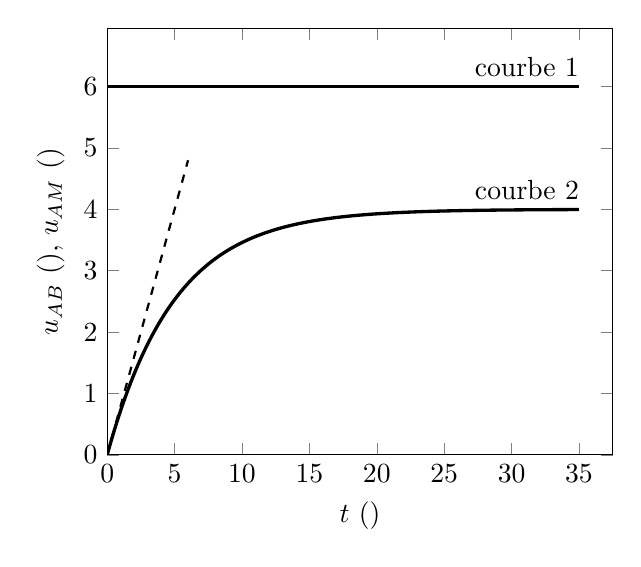
\begin{tikzpicture}
                      \def\A{4}
                      \def\ta{5}
                      \begin{axis}[
                              samples=200,
                              xmin=0,xmax=37.5,
                              ymin=0,ymax=6.95,
                              width=8cm,height=7cm,
                              xtick distance=5,
                              ytick distance=1,
                              xlabel=$t~(\unit{\ms})$,
                              ylabel=
                              {$u_{AB}~(\unit{\volt})$, $u_{AM}~(\unit{\volt})$},
                          ]
                          \addplot[
                                  domain=0:35,
                                  very thick,black
                                  ] {\A*(1-exp(-\x/\ta))}
                                  coordinate[pos=1.02](C1);
                          \addplot[
                                  domain=0:6,
                                  black,thick,dashed
                              ] {\A*\x/\ta)};
                          \addplot[
                                  domain=0:35,
                                  very thick,black
                              ] {6} coordinate[pos=1.02](C2);
                      \end{axis}
                      \node[above left] at (C1) {courbe~2};
                      \node[above left] at (C2) {courbe~1};
                  \end{tikzpicture}
                  \caption{}
                  \label{fig:2bac_svt_national_2017_rattrapage_phys_ex1_3}
              \end{figure}
          \end{minipage}
\end{enumerate}
